\section{Encoding Sets of Attributes} 
\label{sec:flextag_encoding} 
The simplest way to encode a set of attributes is a bitmask with one
bit for each attribute, at the expense of large tags.  In this
section, we present a more concise encoding that uses multiple smaller
bitmasks on different subsets of attributes, at the expense of
slightly larger forwarding tables.  We also present an algorithm
for computing the concise encoding.

%To understand the problem, let us consider a
%simple example for the case of attaching lists of anycast hosts to a packet. Say
%that there is a local area network with five hosts $H = \{h_1, h_2, h_3, h_4,
%h_5\}$, and each packet that arrives will be classified as anycasting to one of
%four possible host sets: $s_1 = \{h_1, h_2\}$, $s_2 = \{h_1, h_2, h_3\}$, $s_3 =
%\{h_1, h_3\}$, or $s_4 = \{h_3, h_4, h_5\}$. In a flat tagging solution to this
%problem, each unique set will be assigned a single tag, and thus a packet which
%can be forwarded to the $i^{th}$ set will receive the $i^{th}$ tag. Now, for an
%intermediate switch to determine, using exact tag matches, if a packet can be
%forwarded to host $h_1$, it must check whether the packet has been assigned to
%$s_1, s_2,$ or $s_3$. The number of entries required is proportional to the
%number of sets which contain $h_1$, in this case 3. In the worst case $h_1$
%would be a member of almost every group, and testing for $h_1$ would required a
%number of checks linear in the number of tags. 

\begin{figure}[t!] \begin{minipage}{1\linewidth}
\begin{subfigure}[b]{0.96\linewidth} 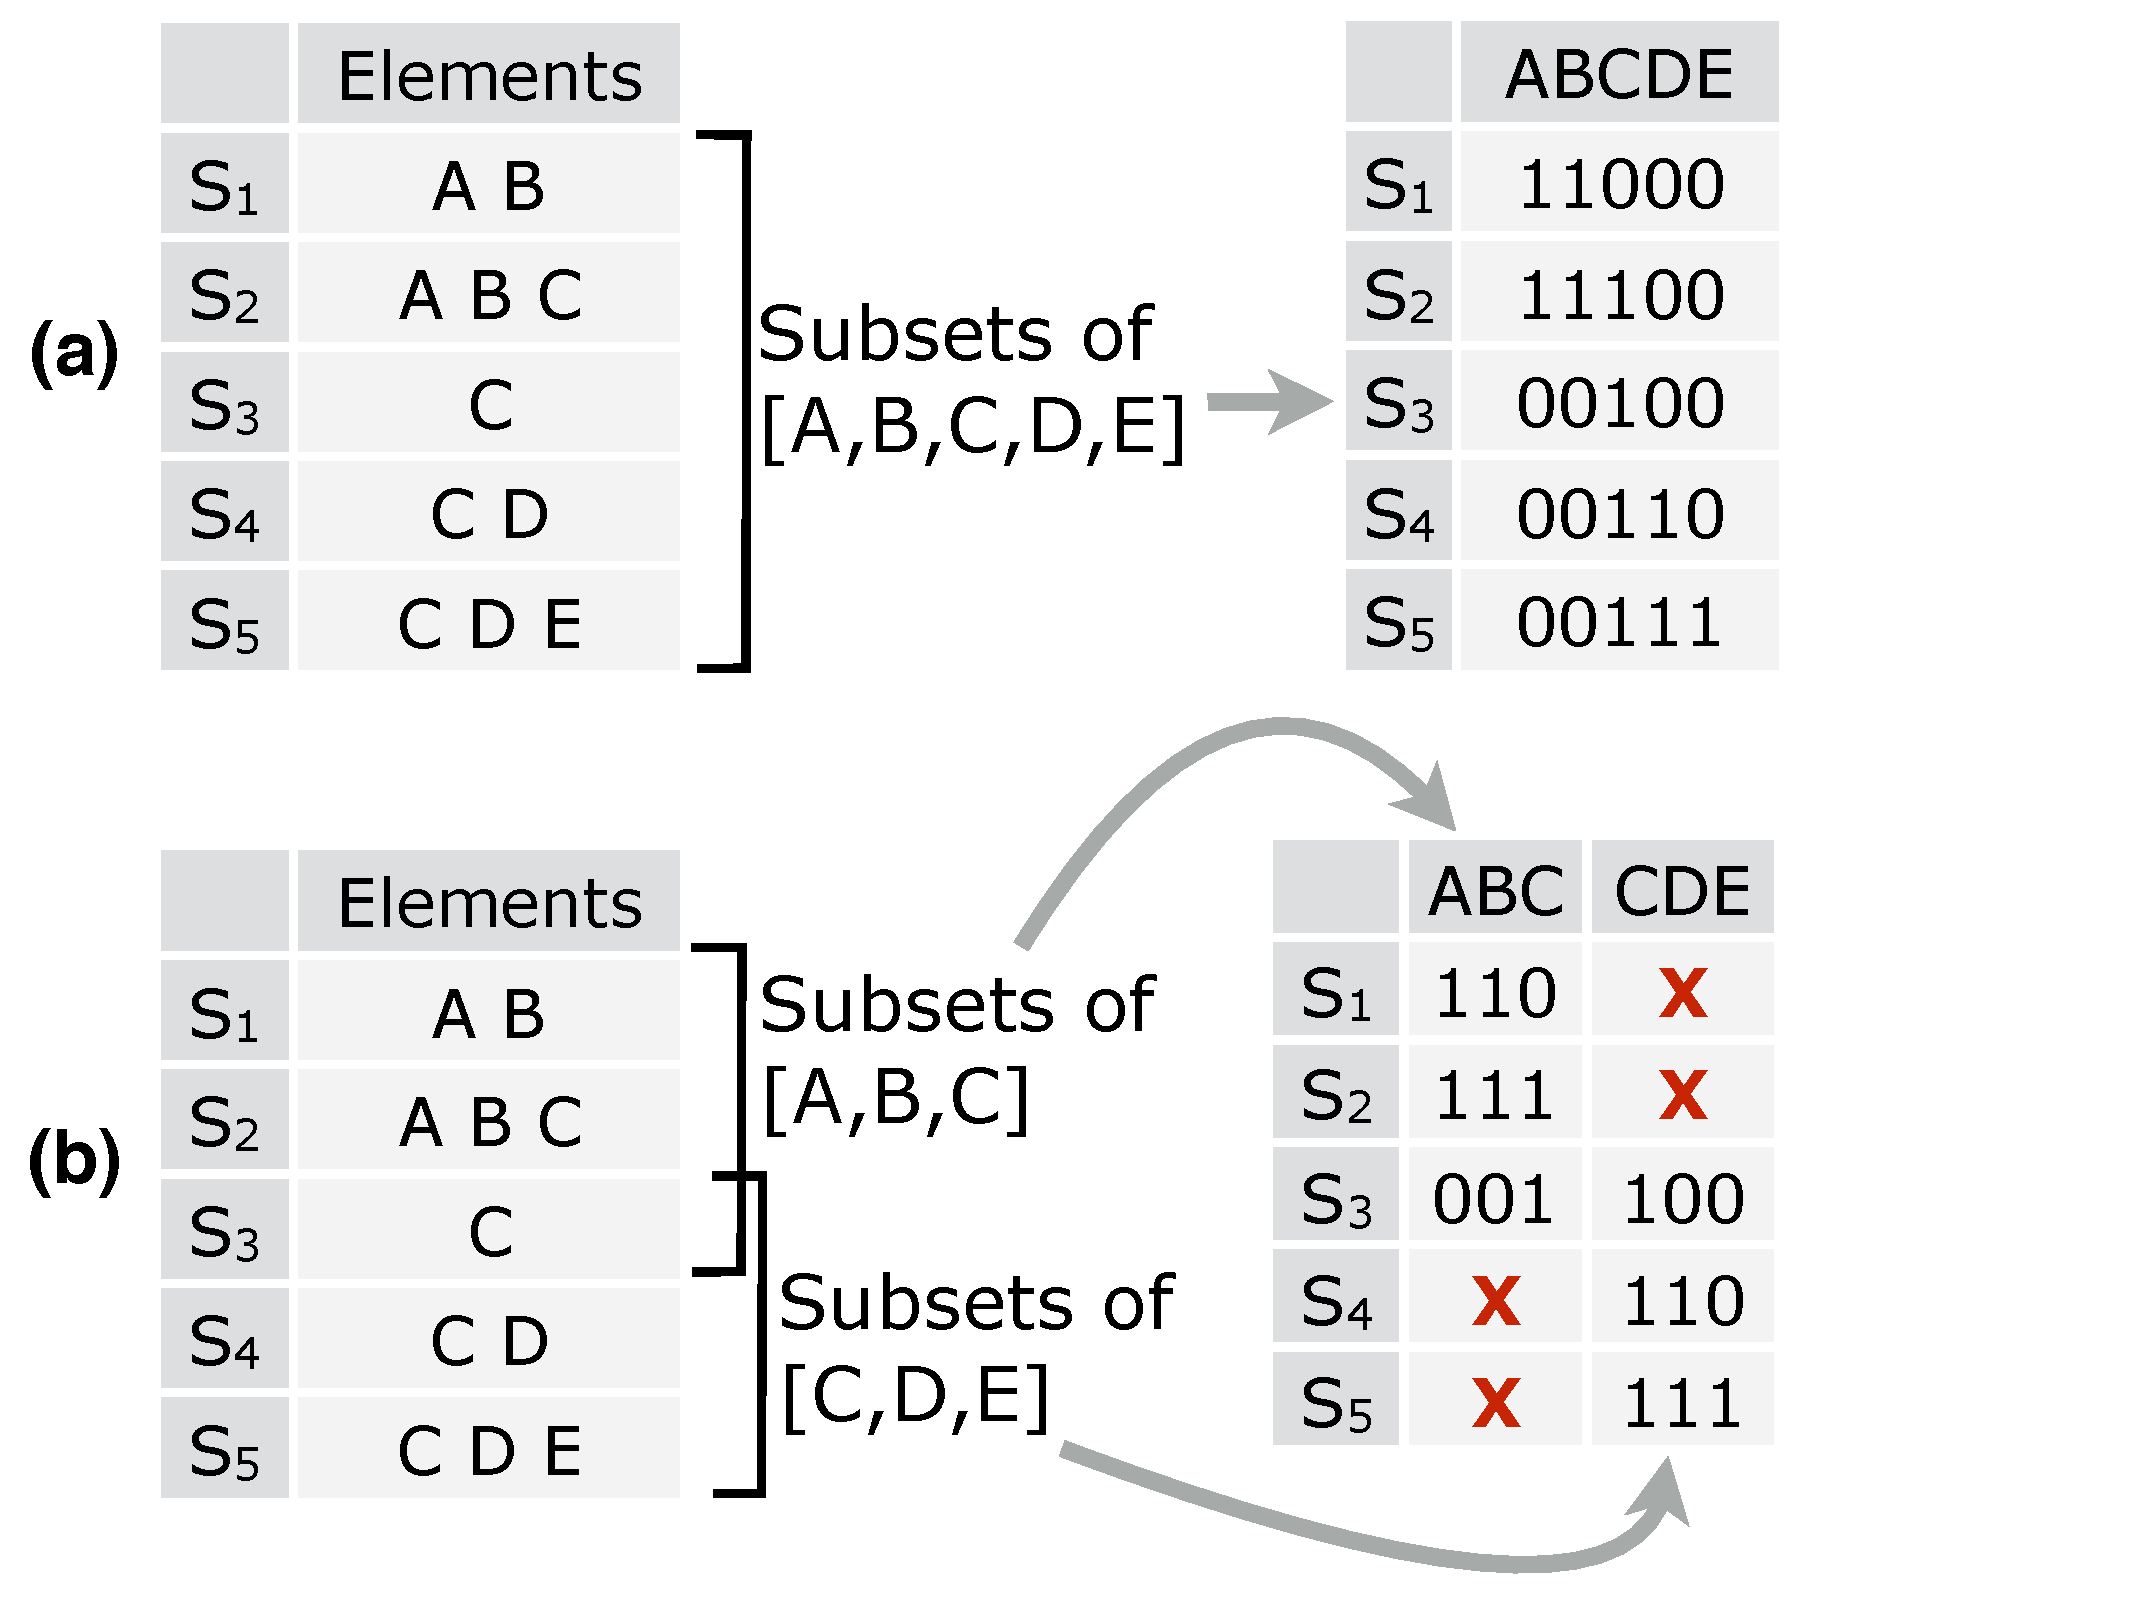
\includegraphics[trim={0 0 5.5cm 0}, clip,
width=\linewidth]{figures/masking} \end{subfigure}
\begin{subfigure}[c]{0.96\linewidth} 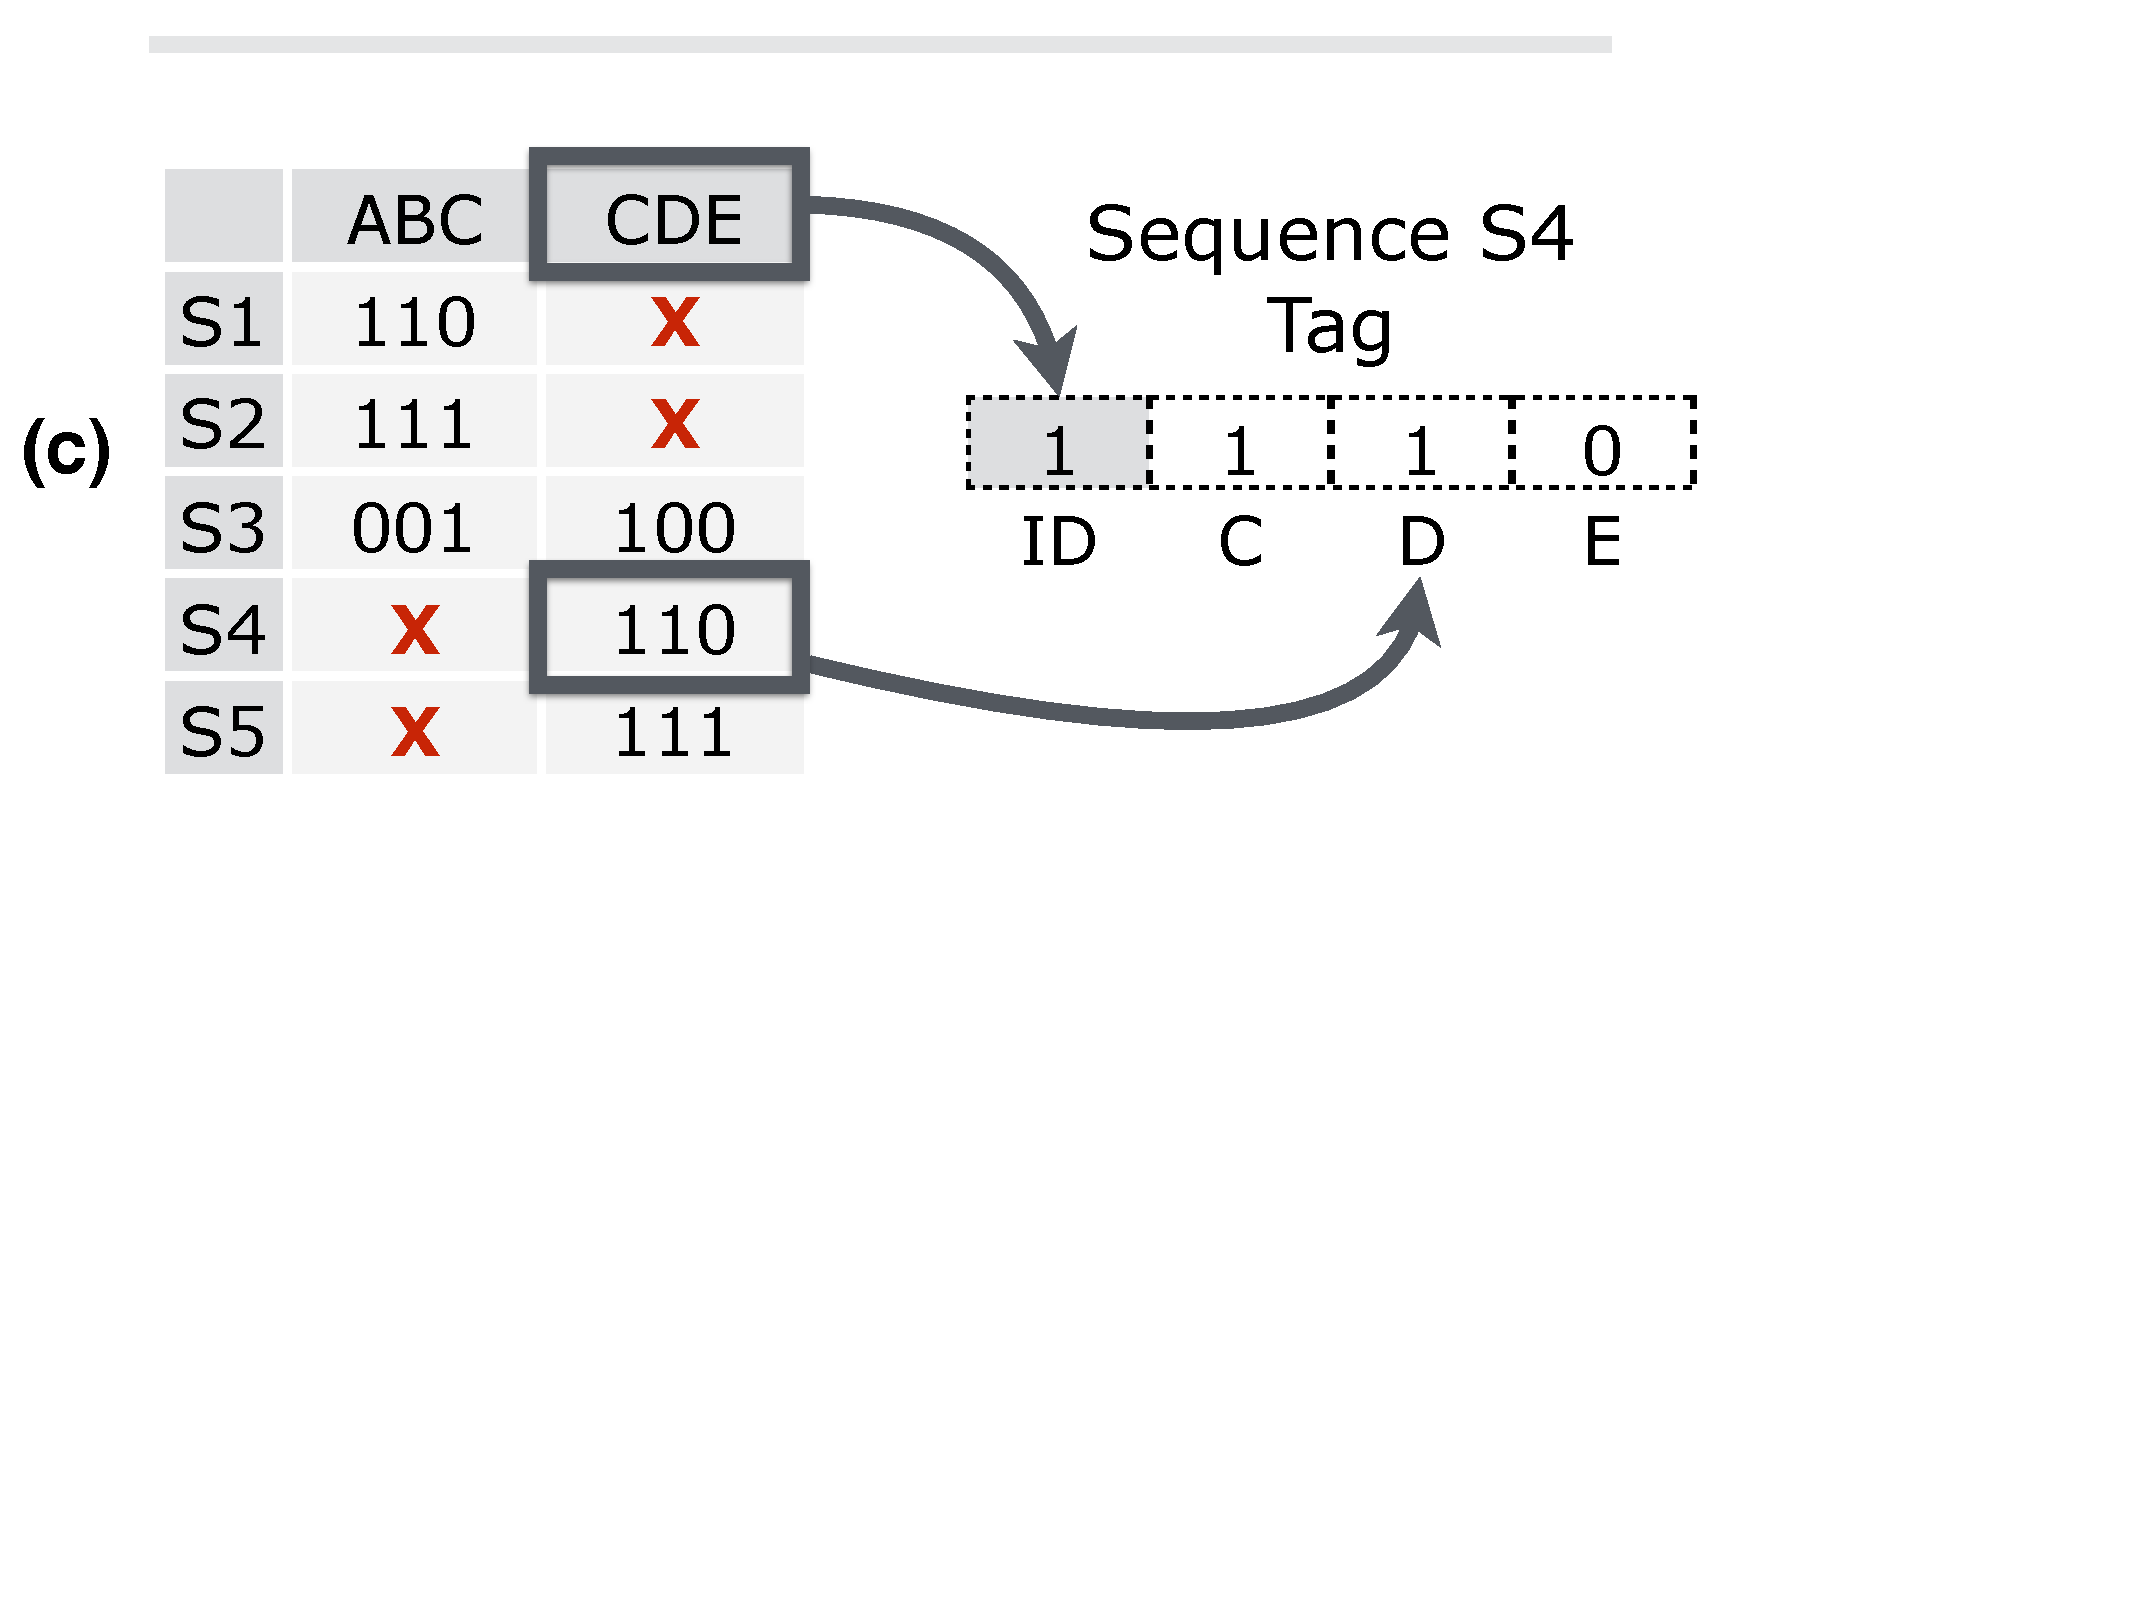
\includegraphics[trim={0 13cm 5.5cm 0},
clip, width=\linewidth]{figures/making_metadata} \end{subfigure} \end{minipage}
\caption{Two different ways to recover attribute sets.
In (a), the sets are recovered by masking over $[A,B,C,D,E]$. In (b), the sets
are recovered by masking over either superset $[A,B,C]$ or set $[C,D,E]$. An X
denotes that the set cannot be fully recovered by masking over the given set.
(c) shows how the matrix in (b) can be mapped to tags.}
\label{fig:masking} \end{figure}

\subsection{Multiple Smaller Subsets of Attributes}
\label{ssec:mset}
%%%
%%% Strawman
%%%
In the strawman solution of a simple bitmask, the tag has one bit for
each attribute.  For example, Figure~\ref{fig:masking}(a) shows
multiple forwarding equivalence classes ($S_1$-$S_5$) that each
correspond to a different subset of five attributes ($A$-$E$), and the
resulting bitmask encoding.  A single forwarding rule can test for any
combination of attributes (e.g., comparing a packet's tag to ``1*1**''
identifies whether attributes $A$ and $C$ hold).  However, when the
number of attributes is large, the tag becomes quite large.

%%%
%%% Concise encoding example in the figure
%%%
Our more concise encoding identifies groups of attributes that
commonly appear together, and creates one shorter bitmask for each
such group.  In the example in Figure~\ref{fig:masking}, attributes
$A$, $B$, and $C$ commonly appear together, as do $C$, $D$, and $E$,
leading to two groups.  The right side of Figure~\ref{fig:masking}(b)
shows how each forwarding equivalence class can be encoded as a
bitmask on $[A,B,C]$, $[C,D,E]$, or both.  To differentiate between
the two groups, the tag can include a one-bit group identifier (e.g.,
a $0$ for $[A,B,C]$ and a $1$ for $[C,D,E]$), as shown in
Figure~\ref{fig:masking}(c).  The result is a four-bit identifier
where, for example, FEC $S_4$ with attributes $C$ and $D$ is encoded
as $1110$.

%%%
%%% Slightly larger forwarding table
%%%
The forwarding rules can match on attributes by considering both the
group id and the associated bitmask.  For example, a switch could test
for attribute $D$ by matching on (i) group identifier $1$ and (ii) the
$D$ bit in group $1$'s bitmask.  Thus, the rule would have a match of
``$1*1*$''.  However, some attributes appear in multiple groups, such
as attribute $C$ in the example.  The switch can use two rules to test
for $C$: (i) ``$0001$'' for group $0$ and (ii) ``$1100$'' for group
$1$.  Thus, our encoding scheme slightly increases the forwarding
table size over the simple bitmask scheme, but only by one rule in
this example.

\subsection{Computing Good Subsets of Attributes}
\label{ssec:merge}




\begin{algorithm}
\DontPrintSemicolon
\KwData{Supersets $\SS$, Tag Width Calculator $W()$, Width Limit $W_{max}$.}
\KwResult{Supersets $\SS$ with minimal memory usage.}
\Begin{
\While{$|\SS| > 1$}{
      	$bestPair \gets (None, None)$\;
      	$bestGain\gets 0$\;
      	\For{$(s_i, s_j) \in \SS\times \SS$}{
      		$\SS_{temp} \gets (\SS-\{s_i, s_j\}) \cup \{s_i\cup s_j\}$\;
      		\If{$W(\SS_{temp}) \le W_{max}$}{
      			$gain \gets \sum_{k \in s_i\cap s_j}q_k$\;
      			\If{$gain > bestGain$}{
      				$bestGain \gets gain$\;
      				$bestPair \gets (s_i, s_j)$\;
      			}
      		}
      	}
      	\If{$bestPair = (None, None)$}{
      		\textbf{break}\;
      	}
      	$(s_a, s_b) \gets bestPair$\;
      	$\SS \gets (\SS-\{s_a, s_b\}) \cup \{s_a\cup s_b\}$\;
      }
      \textbf{return} $\SS$\;
}
\caption{Greedy Memory Minimization\label{alg:memory_min}}
\end{algorithm}


This tag format allows us to test for the presence of many attribute tag using
only a single matching string in switch memory.  However, this is not true for
all attributes. Looking again at Figure \ref{fig:masking}(b), the case of
testing for attribute $C$ is not so simple. Since $C$ appears in both supersets,
we must check whether $C$'s bit is 1 in either superset mask, using the wildcard
strings $["0**1", "11**"]$. In general, any attribute $a$ that appears in $k_a$ supersets
requires $k_a$ wildcard strings to be queried, where the strawman approach
required exactly 1 wildcard string for every attribute. We refer to this effect as inflation. In the Figure
\ref{fig:masking}(b) example, we can eliminate inflation by merging the
supersets $[A,B,C]$ and $[C,D,E]$ into $[A,B,C,D,E]$. No attribute will appear
in multiple sets, but the tag size has increased from 4 to 5 bits (the mask went
from 3 to 5, and the identifier size went from 1 to 0). Note that this is identical to the strawman solution, but it is not the case that only the strawman solution eliminates inflation. If the intersection between the attributes of every pair of sets is empty, then the number of wildcard strings per attribute is always 1, regardless of how many supersets there are. 

However, there may not be an even number of tests per attribute in a network policy, causing inflation
to be less tolerable for some attributes. 
If an attribute $a$ is tested $q_a$ times and appears in $k_a$
supersets, there will be $q_a\cdot k_a$ match strings for that
attribute. If we have a set of supersets $\SS = \{s_1, s_2, \dots, s_N\}$, we
can decrease the amount of memory we will use by replacing any pair
of sets $\{s_i, s_j\}$ in $\SS$ with their union $s_i\cup s_j$. If we do this,
note that the memory used will decrease by $\sum_{a \in s_i\cap s_j}q_a$,
because every attribute $a$ in the intersection of $s_i$ and $s_j$ will appear
in one less superset, eliminating $q_a$ tests from memory. We can extend this
observation to a simple greedy algorithm, which repeatedly finds a pair of
supersets to merge which maximally decreases overall memory usage until any
merging operation would case the maximum tag width to be exceeded. 


Algorithm \ref{alg:memory_min} shows this simple greedy memory minimization
algorithm in its entirety. The algorithm takes as input a superset list $\SS =
\{s_1, s_2, \dots, s_N\}$, a tag width calculator $W()$, and a maximum tag width $W_{max}$. Based on the selected identifier type, the width calculator $W(\SS)$ returns $W_f$ or $W_v$, for which closed formulas are provided later in \S \ref{sec:identifiers}.

We have not stated which superset list $\SS$ to use as an input to our
algorithm. It suffices to begin with any list such that, for every attribute set
$A_i$ in the list of sets we need to encode, there is some superset $s_j \in
\SS$ such that $A_i \subseteq s_j$. An obvious choice for $\SS$ is to take the
list of attribute sets we wish to reproduce as our initial superset list. Note
that there may be many pairs of attribute sets $(A_i, A_j)$ such that $A_i
\subseteq A_j$. There is no reason to keep $A_i$ in $S$ in this case, so we
pre-process $\SS$ by removing any attribute set which is a subset of any other. 